\chapter{Autocompletion Techniques}
\label{chap:Backend}

In this chapter we describe the details of our system. Per \Cref{fig:architecture}, our implementation works as a backend that sits between the user interface and a remote SPARQL query endpoint. It takes SPARQL queries as input and returns suggestions for the variables in those queries. Since we are focusing on dealing with large datasets (480 GB for the uncompressed Wikidata dump), direct in-memory storage/query is not possible; rather a specialized on-disk index is required.  Before we describe the details of our backend, we introduce an extended example in order to provide an overview of the system.

\section{Overview}

Let us consider that a user is looking for "siblings that have directed a film together". 
Since the user might not very familiar with the available properties in a dataset such as Wikidata, it would be hard for them to directly specify the properties they require. Since they might not be familiar with SPARQL syntax it might be even harder for them to specify the required query directly on the SPARQL endpoint. Rather they choose to use a graphical query builder, like RDFExplorer~\cite{Vargas2019}. Let us consider that they have built a graph query such as the one in \Cref{fig:siblingsQueryGraph}:

\begin{figure}[H]
    \centering
        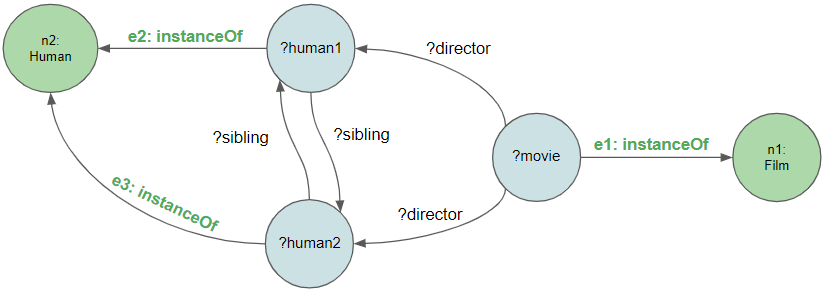
\includegraphics[width=\linewidth]{imagenes/SiblingsGraph.png}
        \caption{Example graph: siblings that have directed a film together}
        \label{fig:siblingsQueryGraph}
\end{figure}

For the example given in \Cref{fig:siblingsQueryGraph}, let us consider that some RDF triples, such as the ones presented in \Cref{fig:siblingsRDFdata}, exist. 

\begin{figure}[H]
\begin{minted}[]{sparql}
[...]
ex:LanaWachowski ex:instanceOf ex:Human . 
ex:LanaWachowski ex:siblingOf ex:LillyWachowski . 
[...]
ex:LillyWachoski ex:instanceOf ex:Human . 
ex:LillyWachoski ex:siblingOf ex:LanaWachowski . 
[...]
ex:Matrix ex:instanceOf ex:Movie .
ex:Matrix ex:directedBy ex:LanaWachowski . 
ex:Matrix ex:directedBy ex:LillyWachoski . 
[...]
\end{minted}
\caption{Example of the underlying RDF data for the query in \Cref{fig:siblingsQueryGraph}.}
\label{fig:siblingsRDFdata}
\end{figure}

Depending on the Linked Data source that is used (e.g.: DBPedia, Wikidata) triples may have different identifiers and namespaces. In \Cref{fig:siblingsWikidataRDF} we present the Wikidata representation for these triples.

\begin{figure}[H]
\begin{minted}[]{sparql}
[...]
wd:Q9545711 rdfs:label "Lana Wachowski"@en .
wd:Q9545711 wdt:P31 wd:Q5 . # Instance of Human
wd:Q9545711 wdt:P3373 wd:Q9544977 . #Sibling Lilly Wachowski
[...]
wd:Q9544977 rdfs:label "Lilly Wachowski"@en .
wd:Q9544977 wdt:P31 wd:Q5 .  # Instance of Human
wd:Q9544977 wdt:P3373 wd:Q9545711 . #Sibling Lana Wachowski
[...]
wd:Q83495 rdfs:label "The Matrix"@en .
wd:Q83495 wdt:P31 wd:Q11424 .  # Instance of Film
wd:Q83495 wdt:P57 wd:Q9545711 . # Director Lana Wachowski
wd:Q83495 wdt:P57 wd:Q9544977 . # Director Lilly Wachowski
[...]
\end{minted}
\caption{Example of the Wikidata RDF data representation of \Cref{fig:siblingsRDFdata}: proper identifiers and namespaces are used.}
\label{fig:siblingsWikidataRDF}
\end{figure}

Without knowing the resource identifiers, or knowing a few of them, and using the Wikidata Query Service~\cite{wikidataQueryService} a user might create a query that could be something like in \Cref{fig:siblingsSPARQL}. 
For the example query, we have added some basic identifiers, such as \texttt{wdt:P31} (\textit{instanceOf}), \texttt{wd:Q5} (\textit{Human}) and \texttt{wd:Q11424} (\textit{Film}), but these might also be variables\footnote{We differentiate constant from variables: a constant in our example would be Human (Q5) or instance of (P31). All the other elements, starting with '?' are variables. Our system will propose results only for variables.}. 
In such a case, users could search values to replace variables via keyword lookup (or leave them as variables and use our system to select a value). 
We have added these values to further explain our backend. We have also added some properties, such as \texttt{?sibling} and \texttt{?director} as variables; we will explain how a user can get suggestions for these variables.
We remark that in practice these variables will likely have generic labels such as \texttt{?var1}, \texttt{?var2}, etc., where we add variables with more intuitive labels for illustration purposes. 
Furthermore, we would also like to note that some relations, like director, can be tricky. One could think that the relation is in the other way: e.g.: \texttt{?human directed ?movie}. We will discuss more about this in our future work \Cref{chap:futureWork}.

\begin{figure}[H]
\begin{minted}[]{sparql}
SELECT * WHERE {
    # ?human1 and ?human2 are instances of (P31) Human (Q5)
    ?human1 wdt:P31 wd:Q5 .
    ?human2 wdt:P31 wd:Q5 .
    
    # ?movie is an instance of (P31) Film (Q11424).
    ?movie wdt:P31 wd:Q11424 .
    
    # ?human1 and ?human2 are ?siblings.
    ?human1 ?sibling ?human2 .
    ?human2 ?sibling ?human1 .
    
    # ?movie has as ?director both ?human1 and ?human2.
    ?movie ?director ?human1 .
    ?movie ?director ?human2 .
}
\end{minted}
\caption{Without some knowledge of the underlying RDF data, a user could create a query where the properties are variables. A query like this will time out in a SPARQL endpoint such as \url{https://query.wikidata.org/}}
\label{fig:siblingsSPARQL}
\end{figure}

The purpose of our system will be to guide users in going from the previously constructed query in \Cref{fig:siblingsSPARQL} to a more complete query such as in \Cref{fig:siblingsSPARQLFull}.

\begin{figure}[H]
\begin{minted}[]{sparql}
SELECT * WHERE {
    # ?human1 and ?human2 are a Human (Q5), ?movie is a Film (Q11424).
    ?human1 wdt:P31 wd:Q5 .
    ?human2 wdt:P31 wd:Q5 .
    
    ?movie wdt:P31 wd:Q11424 .
    
    # ?human1 and ?human2 are siblings (P3373).
    ?human1 wdt:P3373 ?human2 .
    ?human2 wdt:P3373 ?human1 .
    
    # ?movie was directed by (P57) both ?human1 and ?human2.
    ?movie wdt:P57 ?human1 .
    ?movie wdt:P57 ?human2 .
}
\end{minted}
\caption{Our system can provide users with suggestions for entities and properties, so that they can easily identify resources.}
\label{fig:siblingsSPARQLFull}
\end{figure}

Our system can also provide suggestions for \texttt{?human1}, \texttt{?human2} and \texttt{?movie} (such as \textit{Lana Wachowski}, \textit{Lilly Wachowski} and \textit{The Matrix}); which is not what we need in the current scenario, but could be in other scenarios. Once a query is shaped as presented in \Cref{fig:siblingsSPARQLFull}, it can be evaluated to get values for these variables. The query expressed in \Cref{fig:siblingsSPARQLFull} can be run directly on a SPARQL endpoint such as \url{https://query.wikidata.org/} and to date, 125 siblings will be displayed as results. Likewise, we could in theory run the query in \Cref{fig:siblingsSPARQL} over the SPARQL endpoint to generate results, and thus return suggestions for replacing individual variables towards constructing the query of \Cref{fig:siblingsSPARQLFull}. However, the query of \Cref{fig:siblingsSPARQL} times out on the public Wikidata endpoint: with so many variables, it generates too many intermediate results for the endpoint to process in the time limit of 50 seconds. For this reason we propose methods to generate approximate suggestions to replace individual variables of such queries.

For our system to work (in order to get from \Cref{fig:siblingsSPARQL} to \Cref{fig:siblingsSPARQLFull}), first our specialized index must be built and then queries will be processed. Our index differs from a SPARQL endpoint index in that for each triple's \textit{property}, our index does not store the values of the \textit{entities} linked to that \textit{property}, but rather the \textit{types} of those \textit{entities}. This removes the one-to-one relation in triples, thus creating approximations of the possible available values while improving query times.

Our system will actually build two indexes. The first is an \textit{entities} index with the structure shown in \Cref{fig:siblingsEntityIndex}. For each resource we will add a database entry. In the example of \Cref{fig:siblingsEntityIndex}, the `...' as in line 1, are to show that our data could have other values not listed in the example. 
\begin{figure}[H]
\begin{minted}[]{css}
LanaWachowski.Type = [Human,...]
LanaWachowski.Properties = [instanceOf, siblingOf,...]
LanaWachowski.InverseProperties = [siblingOf, directedBy,...]
[...]
LillyWachoski.Type = [Human,...]
LillyWachoski.Properties = [instanceOf, siblingOf,..]
LillyWachoski.InverseProperties = [siblingOf, directedBy,...]
[...]
Matrix.Type = [Film,...]
Matrix.Properties = [instanceOf, directedBy,....]
Matrix.InverseProperties = [...]
[...]
Human.Type = [...]
Human.Properties = [...]
Human.InverseProperties = [instanceOf,...]
[...]
Film.Type = [...]
Film.Properties = [...]
Film.InverseProperties = [instanceOf,...]
\end{minted}
\caption{Representation of the entity index for the \Cref{fig:siblingsRDFdata} data.}
\label{fig:siblingsEntityIndex}
\end{figure}

Afterwards, a \textit{properties} index will be built as in \Cref{fig:siblingsPropertyIndex}. As before, we are adding `...' on the fields to show that our fields could have additional values not included in our example.
\begin{figure}[H]
\begin{minted}[]{css}
siblingOf.Domain = [Human,...]
siblingOf.Range = [Human,...]
[...]
director.Domain = [Film,...]
director.Range = [Human,..]
[...]
instanceOf.Domain = [Human, Film,...]
instanceOf.Range = [...]
\end{minted}
\caption{Representation of the property index for the \Cref{fig:siblingsRDFdata} data.}
\label{fig:siblingsPropertyIndex}
\end{figure}

Once the index is built, queries can be processed. Given a query graph, our system will first check all the graph's nodes and edges for constants. For each constant element, we will annotate that element: nodes with the types of that constant; and edges with the constant's domain- and range-types (as seen on \Cref{chap:motivation}). 

From our example, we know the following:

\begin{minted}[escapeinside=||,frame=none,linenos=false]{text}
|\bf{Constants:}|
Human (Q5)
Film (Q11424)
InstanceOf (P31)

|\bf{Variables:}|
?human1
?human2
?movie
?sibling
?director
\end{minted}

Since we know some constants, we have information about the types of some nodes and edges. This gives our system some data about variable-nodes and -edges linked to known constants. 

\begin{minted}[escapeinside=||,frame=none,linenos=false]{text}
|\bf{Types:}|
?human1 is Human
?human2 is Human
?movie is Film
\end{minted}

At this point, we can provide approximated suggestions for every element that links to our known constants. The next step is to retrieve the domain- and range-types for our variables from our index over the data. 

\begin{minted}[escapeinside=||,frame=none,linenos=false]{text}
|\bf{Domain and range types:}|
?sibling has domain Human and range Human.
?director has domain Film and range Human.
\end{minted}

Additionally, our database might contain several domain- and range-types for constant properties:

\begin{minted}[escapeinside=||,frame=none,linenos=false]{text}
mother (P25), spouse (P26), child (P40) have domain Human and range Human.
producer (P162) has domain Film and range Human.
studiedAt (P69) has domain Human.
ownedBy (P127) has range Human.
genre (P136) has domain Film.
basedOn (P144), derivativeWork (P4969) have range Film.
\end{minted}

Our system will evaluate the domain and range types of our inferred values:
\begin{minted}[escapeinside=||,frame=none,linenos=false]{text}
Human.Domain = [sibling, mother, child, studiedAt, ...]
Human.Range = [sibling, mother, child, ownedBy, ...]
Film.Domain = [director, producer, genre, ...]
Film.Range = [basedOn, derivativeWork, ...]
\end{minted}

In order to get proper suggestions, we need to intersect the inferred types and provide relevant suggestions for those inferred values. Intersecting types is required to match the information we know about linked constants. If a node, for instance, has incoming and outgoing edges, the possible types of that node will be the ones that are a match for all of those incoming and outgoing edges. Since we may know the domain- and range-types of some properties of those edges, we can estimate that the possible types for a node would be those in the intersection of the incoming-edges-range-types and the outgoing-edges-domain-types.

\begin{minted}[escapeinside=||,frame=none,linenos=false]{text}
|\bf{Suggestions:}|
?sibling = [mother (P25), child (P40), sibling (P57), ...]
?director = [director (P57), producer (P162), ...]
\end{minted}

With these suggestions at hand, a user can select the values that they are looking for, instead of trying to figure out the structure of the RDF data that they are querying for.

We will now proceed to explain the details of our backend. The system is composed of four modules, here ordered by their relevance to the system: 
the entities and properties index,
a query parser module,
a graph exploration module and
a query execution module. 
An additional application interface (API) acts as the entry point for our system.

This chapter starts off by detailing the specialized index.
The index section includes the pre-processing and indexing of an RDF dataset dump.

We will then proceed by describing the graph parser module, which converts an input to our own data structure. 
In our case, a graph data structure is used to store our SPARQL statements. 
In this graph, the nodes will represent statements' \textit{subjects} and \textit{objects}, while edges are labelled with \textit{predicates}. 

This graph is then processed by the graph exploration module. 
At this stage, basic information about the nodes, edges and certain relations between them are identified and added to the data structure. 
With this information in place, the graph is passed on to the query execution module. 

The execution of the query is sent in parallel to both the remote SPARQL endpoint and the local index. 
The request to the remote endpoint is sent with a configurable timeout, usually of a few seconds. 
If the remote SPARQL endpoint returns values within this time, these results will be returned; otherwise, the specialized local index results will be post-processed and returned. 

The local index will return information about certain \textit{types}, \textit{entities} and \textit{properties}. 
These results will be processed; mainly some intersections and duplication removal is required at this stage.
The post-processed results are then sent back to the user for display and selection.

This double request mechanism allows us to deliver exact results in the case that the remote SPARQL endpoint does not time out, or otherwise, the over-approximated results from our local index in case it does time out. 
Thus, the system can return possible results that would otherwise keep the user indefinitely waiting or in the worst case, never return. 

The chapter concludes by describing our application interface, which works as the entry point of our system. 
It will take requests from different services, such as SPARQL query editors or SPARQL visual explorers and send the information either to the graph parsing module, for SPARQL queries; 
or directly to the index, for keyword search. 
The integration with a user interface will be left for \Cref{chap:Frontend}.

% ##############################################################################################
% ##############################################################################################
% ##############################################################################################

\section{Initialization}
\label{chap:init}

Before indexing the data, some pre-processing is required. 
The pre-processing filters what are considered valid triples and adds certain inverse relations between some triples that are read. 
The system will process an RDF dump to make the following changes to it:
\begin{itemize}
    \item Filter valid triples.
    \item Add inverse relations.
    \item Sort the file.
\end{itemize}

\begin{figure}[H]
    \centering
        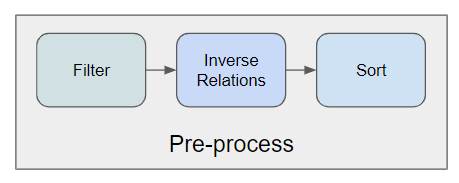
\includegraphics[width=0.5\linewidth]{imagenes/Preprocess.png}
        \caption{Pre-processing workflow}
        \label{fig:preprocess}
\end{figure}

Another important aspect of the system is that it takes compressed files as inputs, and generates compressed output files. 
This is important mainly due to space restrictions. 
The Wikidata dump\footnote{As of February 2020} is $\sim$36 GB compressed and $\sim$480 GB decompressed.
A pre-processed output file is $\sim$8 GB compressed. 

\subsection{Filter}

The first pre-processing task is to filter the input data. 
We will focus on Wikidata labels and descriptions in the English language. 
We will also remove triples with datatype values or external IDs.
While this step could be optional depending on the use-case, the RDFExplorer system that we currently support does not consider such values, and filtering them, currently helps to reduce the number of triples that the system will have to index later. 
Multiple filtering criteria are implemented in the system. 
At the current development stage, these criteria are hard-coded, but they could be extended to use regular expressions or other types of filtering rules. We have left this as a point of future work.

We include triples that match the following rules in our data:
\begin{itemize}
    \item Where \textit{subject} starts with \texttt{http://www.wikidata.org/entity/}.
    \item Where \textit{predicate} starts with \texttt{http://www.wikidata.org/prop/direct/} 
            \subsubitem and \textit{object} starts with \texttt{http://www.wikidata.org/entity/}.
        \subitem or \textit{predicate} is \texttt{label}, \texttt{description} or \texttt{alt-label} 
            \subsubitem and \textit{object} is \textit{literal} and ends with \texttt{@en}.
\end{itemize}

\begin{example}
We now present some examples of both filtered and non-filtered triples.
We have used prefixes when required for shortening lines.

Examples of triples that are kept:
\begin{minted}{SPARQL}
#Entity or Property Subject, Label predicate in english:
wd:Q27 rdfs:label "Ireland"@en .
#Entity or Property Subject, Description predicate in english:
wd:Q147 schema:description "young of a cat"@en .
#Entity or Property Subject, Alternative Label predicate in english:
wd:P22 skos:altLabel "dad"@en .
#Entity subject, Property predicate, Entity subject triples:
wd:Q465 wdt:P277 wd:Q251 .
\end{minted}

Examples of triples that are removed:
\begin{minted}{SPARQL}
#Non-english literal objects:
wd:Q27 rdfs:label "Irlanda"@it .
#Non -Label, -Description or -AltLabel predicates:
wd:Q298 skos:prefLabel "Chile"@en .
wd:Q348 <http://www.wikidata.org/prop/direct-normalized/P349> <object> .
#Non-Entities or -Property subjects:
<http://wikiba.se/beta#Dump> <http://schema.org/softwareVersion> "0.1.0" .
<https://www.wikidata.org/wiki/Special:Entity/Q27> rdfs:label "Irland"@en .
#Non-literal or -entity objects:
wd:Q47 wdt:P1082 "1852168"^^<http://www.w3.org/2001/XMLSchema#decimal> .
\end{minted}
\end{example}

\subsection{Inverse relations and sorting}

Following the filtering process, the system adds the inverse relation for triples patterns containing non-literal objects. 
For every \texttt{(subject, predicate, object)} triple with only non-literal \texttt{objects}, the system adds the inverse \texttt{(object, inverse/predicate, subject)} triple. This will allow us to treat the subject and object positions of triples equally for the purposes of generating suggestions, while requiring minimal additional code in later components.

\begin{example}
For example, the following triples:

\begin{minted}{SPARQL}
<uri:/subjectA> <uri:/type> <uri:/subjectTypeB> .
<uri:/subjectA> <uri:/predicate> <uri:/objectC> .
\end{minted}

Produces a new file with the original triples, plus the new inverse relation triples:

\begin{minted}{SPARQL}
<uri:/subjectA> <uri:/type> <uri:/subjectTypeB> .
<uri:/subjectA> <uri:/predicate> <uri:/objectC> .
[...]
<uri:/subjectTypeB> <uri:/inverse/type> <uri:/subjectA> .
[...]
<uri:/objectC> <uri:/inverse/predicate> <uri:/subjectA> .
\end{minted}

The separation $[...]$ between \textit{subject}, \textit{object} and \textit{subjectType} statements are due to the final pre-processing task: sorting the output dump file. 
This keeps entity related triples grouped together, which in turn makes indexing more efficient.

\end{example}

The second benefit of this approach, is that with this sorting, finding if an \textit{entity} is a \textit{type} is immediate, since it will contain predicates as \textit{/inverse/type} within its triples. 
The pre-processing could exclude this step; nevertheless, adding the inverse triples significantly reduces indexing time, while without it, several iterations through disk access would have been required. 

The final step is to sort the pre-processed file. Sorting is done via merge sort. At the current development stage, the process is called from the command line. It is to be noted that for sorting of the file, $\sim$3$\times$ the size of the input file is required as free disk space. The command used for sorting is as follows: 

\begin{minted}[frame=none]{bash}
    gzip -dc {input} | LANG=C sort                      \
         -S 200M                                        \
         --parallel=4                                   \
         -T tmp/                                        \
         --compress-program=gzip | gzip > {output}
\end{minted}

This command takes an \texttt{\{input\}} compressed file as parameter. It sorts it using the \texttt{tmp/} folder for storing temporary files, where each chunk during the merge-sort process is as large as 200 Mbytes. During the process, it uses 4 threads. Finally, the sorted results are compressed to an \texttt{\{output\}} file.

% ##############################################################################################
% ##############################################################################################
% ##############################################################################################

\section{Index}
\label{chap:index}

After a pre-processed dump has been created, the system can start indexing it. 
Indexing occurs in two steps: once for entities and once for properties. In the end, two indexes are created, one for each.

Entity indexing involves the following steps:
\begin{itemize}
    \item Rank entities via PageRank
    \item Index entities
\end{itemize}

Properties indexing has the following steps:
\begin{itemize}
    \item Rank properties by frequency
    \item Build a domain dictionary
    \item Build a range dictionary
    \item Index properties
\end{itemize}

A depiction of both of these processes can be seen in \Cref{fig:indexing}.

\begin{figure}[H]
    \centering
        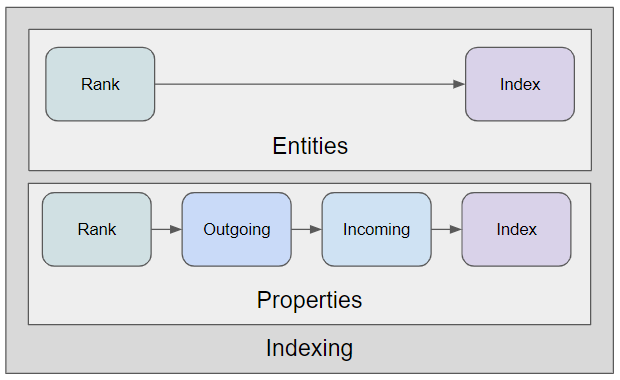
\includegraphics[width=0.7\linewidth]{imagenes/Indexing.png}
        \caption{Indexing workflow}
        \label{fig:indexing}
\end{figure}

\subsection{Entities}

\subsubsection{Inverted Index}

Data relating to entities is indexed using \textit{Lucene}. 
As discussed in \Cref{chap:lucene}, Lucene is a search engine library, mostly suitable for text indexing and searching capabilities. 
This enables out-of-the-box keyword-search for entities and properties.
As mentioned previously, Lucene adds a relevance metric based on TF-IDF, which complements the PageRank value that we will calculate later.

The index in Lucene is a document database index. 
Each document of this database has fields. 
In our case, each document corresponds to an \textit{Entity} and each \textit{Entity} has fields such as \textit{Label}, \textit{Description} or a collection of \textit{Properties}. 
We now present each \textit{Field} that every Document in our index has, and the description of those \textit{Fields}.

Each entity-document contains the following fields:
\begin{itemize}
    \item \textbf{Id:} String field. The IRI of the entity. In our case, it is stored without the prefix. For Wikidata, this identifier is a letter \texttt{Q} followed by the identification number.
    \item \textbf{Label:} Text field.  Value that represents a name for the resource (that may be ambiguous).  In the Wikidata dump, the label is the value of the triples with the predicate \url{http://www.w3.org/2000/01/rdf-schema#label}. 
    \item \textbf{AltLabel:} Text field. Other names the resource is known by.  The predicate for these values in the dump is \url{http://www.w3.org/2004/02/skos/core#altLabel}. This field can store multiple values for the same document.
    \item \textbf{Description:} Text field. Small description of the resource, which helps to disambiguate the resource from others with the same or similar labels. Triples with a description have the predicate \url{http://schema.org/description}.
    \item \textbf{InstanceOf:} String field. Indicates if the entity is a type. For example, \textit{Barack Obama (Q76)} is type \textit{Human (Q5)}. \textit{Human} has a \textit{InstanceOf} field with a \textit{"true"} value while \texttt{Barack Obama} has an InstanceOf field with \textit{"false"}. This is based on having a property \texttt{inverse/instanceOf (P31)} on at least one incoming edge. This is possible due to adding the previously mentioned inverse relation for properties in the pre-processing stage, which when sorted groups both incoming and outgoing edges for a particular entity.
    \item \textbf{Property:} String field. The collection of the outgoing properties that this resource has. This field can store multiple values. All values in this field are stored without their prefix. Property predicates start with  \url{http://www.wikidata.org/prop/direct/}
    \item \textbf{InverseProperty:} String field. Same as the Property field, but for incoming properties. As was mentioned before, these triples were added in the pre-processing step to the dump file.
\end{itemize}

\subsubsection{Ranking}

Lucene offers relevance-based ranking (using a variant of TF-IDF) for searches. But we need importance too: a user might be searching for the term `Obama'. The reader might think about \textit{Barack Obama} as a first suggestion; though \textit{Tom Obama} or \textit{Mount Obama} might have the same relevance in terms of TF-IDF and keywords, one result is much more important than the other and thus we assume it to be of higher prior probability to be relevant to the user.

In order to get the results sorted by both relevance and importance, a ranking value, calculated via PageRank, is added to our index. 
As seen in \Cref{chap:pagerank}, PageRank was originally designed for directed graphs such as websites and their links. 
PageRank works by iteratively setting relevance values on nodes based on the incoming and outgoing nodes (edges pointing to other nodes). 
In the same way, our PageRank implementation works by iteratively setting the relevance of incoming and outgoing entities through their edges. 

Our implementation of PageRank works in memory, and is not different from other implementations. 
Due to the amount of data, for our implementation we have considered using value types (e.g.: \texttt{int, double, arrays}) instead of more complex reference types (e.g.: \texttt{List, Dictionary, etc.}) in favor of performance. 
Twenty iterations have been considered for this ranking process.

PageRank values are stored in the index as \textit{Lucene's Boost} value. This helps Lucene to sort the results of a query by their importance, as well as relevance. PageRank values are stored in both the \textit{Label} and \textit{AltLabel} fields.

\begin{example}
As an example, a collection of triples from a single entity is presented. Its indexed document and field representation is also presented. We have taken a partial sample of the Universe (Q1) as an example reference.

\begin{minted}{SPARQL}
wd:Q1 schema:description "totality of space [...]"@en .
wd:Q1 rdfs:label "Universe"@en .
wd:Q1 skos:altLabel "Our Universe"@en .
wd:Q1 skos:altLabel "The Cosmos"@en .
wd:Q1 wdt:P31 wd:Q36906466 .
wd:Q1 wdt:P361 wd:Q3327819 .
wd:Q1 wdt:P793 wd:Q323 .
wd:Q1 wdt:P828 wd:Q323 .
wd:Q1 <http://www.wikidata.org/prop/reverse/P1542> wd:Q323 .
\end{minted}

The index document representation for these triples is shown in \Cref{table:triplesToDocument}.

\begin{table}[h!]
\centering
\begin{tabular}{ll}
Field           & Value                    \\ 
\hline
Id              & Q1                       \\
Label           & Universe                 \\
AltLabel        & Our Universe             \\
AltLabel        & The Cosmos               \\
Description     & totality of space [...]  \\
InstanceOf      & Q36906466                \\
Property        & P361                     \\
Property        & P793                     \\
Property        & P828                     \\
InverseProperty & P1542                   
\end{tabular}
\caption{Document and field representation of example triples describing the universe}
\label{table:triplesToDocument}

\end{table}

\end{example}

\subsection{Properties}
The next step in the initialization stage is to create an index for the properties contained in the input dataset.

\subsubsection{Inverted Index}
As  was done with the \textit{Entities Index}, an \textit{index} for the \textit{properties} in the dump is also created. In this case, each document corresponds to a \textit{property} and each \textit{property} has fields such as \textit{label}, \textit{description} or a collection of \textit{domain} and \textit{ranges}. 
We now present each \textit{field} in our index, and the properties of those \textit{fields}.

Each property-document contains the following fields:
\begin{itemize}
    \item \textbf{Id:} String field. The IRI of the property. In our case, it is  stored without the prefix. For Wikidata, this identifier is a letter \texttt{P} followed by the identification number.
    \item \textbf{Label:} Text field.  Value that represents a name for the resource.  For the properties in the dump, the same predicate (\url{http://www.w3.org/2000/01/rdf-schema#label}) is used for labels. 
    \item \textbf{AltLabel:} Text field. Other names the resource is known by. The predicate for these values in the dump is \url{http://www.w3.org/2004/02/skos/core#altLabel}. As in the entities index, this field can store multiple values for the same document. Frequency relevance values are stored here as well. This helps Lucene to sort the results of a query by their relevance.
    \item \textbf{Description:} Text field. Small description of the resource, which helps to disambiguate the resource from others with the same labels. Triples with a description have the predicate \url{http://schema.org/description}.
    \item \textbf{Domain:} String field. The collection of the entity-types with one or more instances that have one or more edges with the given property directed outwards from them. This field can store multiple values. All values in this field are stored without their prefix.
    \item \textbf{Range:} String field. The collection of the entity-types with one or more instances that have one or more edges with the given property directed inwards towards them. This field can store multiple values. All values in this field are stored without their prefix.
\end{itemize}

\subsubsection{Ranking}
For ranking \textit{Properties}, the frequency of appearance is used as our relevance metric. 
We are using frequency since PageRank, which is good for ranking nodes in a directed graph, is not very good for ranking edge labels.
In order to calculate these values, a \textit{Dictionary} is built with the \textit{Key} being the \textit{PropertyId} and the \textit{Value} being the amount of times this property appears in the dataset.

Frequency relevance values are used as \textit{Lucene's Boost}, which are multiplied with the reference scores computed based on TF-IDF. This helps Lucene to sort the results of a query by relevance. The Boost values are added again to both \textit{Label} and \textit{AltLabel} fields.

\subsubsection{Type Domains}

Given a triple pattern statement, \textit{Type Domains} allow the system to provide suggestions in the following two scenarios:
\begin{itemize}
    \item Given a \textit{Property}: the system provides suggestions for the \textit{Subject}.
    \item Given a \textit{Subject}: the system provides suggestions for the \textit{Property}.
\end{itemize}

\textit{Type Domains} work by creating a \textit{Dictionary} with \textit{PropertyId} as \textit{Key} and all the \textit{TypeIds} that each \textit{Property} has as \textit{Domain}.

\begin{example}
Given the following data:
\begin{minted}[frame=none,linenos=false]{SPARQL}
<uri:/BarackObama> <uri:/instanceOf> <uri:/Human> .
<uri:/BarackObama> <uri:/bornIn> <uri:/Honolulu> .
\end{minted}

And given the following triple pattern:
\begin{minted}[frame=none,linenos=false]{SPARQL}
?var1 <uri:/bornIn> ?var2 .
\end{minted}

As suggestions for \texttt{?var1} the system provides instances of \texttt{Human} as suggestions, sorted by relevance. Among the results \texttt{BarackObama} can be found.

This type of query usually times out when run on the remote endpoint (when no or a not low enough \texttt{LIMIT} statement is present) and will not offer ranked options. Our claim is that this feature of our system will provide users with ranked suggestions in a predictable amount of time.
\end{example}

\begin{example}
Given the following data:
\begin{minted}[frame=none,linenos=false]{SPARQL}
<uri:/BarackObama> <uri:/instanceOf> <uri:/Human> .
<uri:/BarackObama> <uri:/bornIn> <uri:/Honolulu> .
\end{minted}

And given the following triple pattern:
\begin{minted}[frame=none,linenos=false]{SPARQL}
<uri:/BarackObama> ?prop1 ?var2 .
\end{minted}

As suggestions for \texttt{?prop1} the system provides properties that direct outwards from instances of \texttt{Human}, sorted by frequency. Among the results \texttt{bornIn} can be found.

It is worth mentioning that for this scenario, the baseline system queries the remote endpoint, which returns the properties only available for \texttt{BarackObama}. In case that this query fails, our system would do as mentioned before and return the approximated results from our local index.
\end{example}

\subsubsection{Type Ranges}

Given a triple pattern statement, type ranges allow our system to provide suggestions in the following two scenarios:
\begin{itemize}
    \item Given a \textit{Property}: the system provides suggestions for the \textit{Object}.
    \item Given an \textit{Object}: the system provides suggestions for the \textit{Property}.
\end{itemize}

\textit{Type Ranges} work similarly as \textit{Type Domains}: by creating a \textit{Dictionary} with \textit{PropertyId} as \textit{Key} and all the \textit{TypeIds} that each \textit{Property} has as \textit{Range}.

\begin{example}
Given the following data:
\begin{minted}[frame=none,linenos=false]{SPARQL}
<uri:/BarackObama> <uri:/bornIn> <uri:/Honolulu> .
[...]
<uri:/Honolulu> <uri:/instanceOf> <uri:/City> .
\end{minted}

And given the following triple pattern:
\begin{minted}[frame=none,linenos=false]{SPARQL}
?var1 <uri:/bornIn> ?var2 .
\end{minted}

As suggestions for \texttt{?var2} the system provides instances of \texttt{City} as suggestions, sorted by relevance. Among the results \texttt{Honolulu} can be found.

This type of query times out on a SPARQL endpoint in most cases. As in the \textit{Type Domain} example, we claim that this indexed feature will once again provide users with ranked suggestions in a predictable amount of time.
\end{example}

\begin{example}
Given the following data:
\begin{minted}[frame=none,linenos=false]{SPARQL}
<uri:/BarackObama> <uri:/bornIn> <uri:/Honolulu> .
[...]
<uri:/Honolulu> <uri:/instanceOf> <uri:/City> .
\end{minted}

And given the following triple pattern:
\begin{minted}[frame=none,linenos=false]{SPARQL}
?var1 ?prop1 <uri:/Honolulu> .
\end{minted}

As suggestions for \texttt{?prop1} the system provides properties that point to instances of \texttt{City}, sorted by frequency. Among the results \texttt{bornIn} can be found.

In contrast to what was described for the type domains, our experience has shown that these values are not always returned before a timeout from the remote endpoint since in Wikidata, objects such as cities, countries, types, etc., may have very high in-degree. This feature of our system will provide users ranked suggestions in a predictable amount of time.
\end{example}

\section{Query Parser}
\label{chap:parser}

Once both entities and properties have been indexed, the system can go into online mode. After receiving a user request, the first action of the system is to parse the given request.

We have previously mentioned that the system can work in two ways: keyword search and query term suggestions. Keyword search is quite straightforward: a keyword is given and the inverted index searches and returns the relevant values. These requests go directly to the inverted index, which in turn returns the desired results. No further processing is involved.

Regarding the query term suggestions, there are two possible inputs that the system can take:
\begin{itemize}
    \item \textbf{Query as a graph:} A graph object is passed to our system. This integrates better with graphical user interfaces, such as RDFExplorer.
    \item \textbf{Query as text:} A SPARQL query is passed to our system. This approach is most suitable for text query clients, such as the Wikidata Query Endpoint.
\end{itemize}

For both query term suggestion cases, the goal of the \textit{Query Parser} is to convert the input into a graph data model.

In SPARQL query input scenarios, the input query text is converted using the following triple pattern rules:
\begin{itemize}
    \item Only \texttt{SELECT WHERE} queries are supported in the current version. The system will ignore the \texttt{SELECT} variables (since suggestions can be generated for both projected and unprojected variables when building the query) and take the \texttt{WHERE} statements.
    \item Each triple pattern statement follows a \texttt{Subject Predicate Object} construction.
    \item Each term can be either a constant or a variable.
    \item Each variable will start with the question mark character \texttt{?}. E.g.: \texttt{?var1, ?prop7}
    \item Each constant can be either an IRI in the form of \texttt{<http://iri>} or \texttt{prefix:iri}, when the prefix is given.
\end{itemize}

Given such inputs, parsing an incoming request is straightforward and the queries are converted to the input graph.

% ##############################################################################################
% ##############################################################################################
% ##############################################################################################

\section{Graph Exploration}
\label{chap:graph_exploration}

After a request has been received and the data has been converted into the graph data model, the system explores this graph to check existing relations between nodes and edges. 

The first step of the graph exploration process checks the following:
\begin{itemize}
    \item Which nodes and edges are variables and which are constants.
    \item Which variable nodes have an \texttt{instanceOf} outgoing edge.
\end{itemize}

As a first step, all edges are marked as constant or variable: 
if an edge has a URI as its property, then that edge is considered constant; otherwise it is considered to be variable. 
All nodes are checked in the same manner: if a node has a provided URI, then that node is considered to be a constant, otherwise it is considered to be a variable. 

The next step is to mark the variable nodes as \texttt{Typed}:
If a node is the source of an \texttt{instanceOf} property edge with a target constant, then the node is considered to be \texttt{typed}. To expand on this, let us consider the following statement: \texttt{?var1 instanceOf Human}. As a remark for this case, no other incoming and outgoing edges are available for \texttt{?var1}. We can then consider \texttt{?var1} to have the type \texttt{Human}.

We can summarize this graph exploration with the pseudo-code shown in \Cref{fig:codeExploration}.
\begin{figure}[H]
\begin{minted}[]{csharp}
ExploreGraph (graph) {
  //We will start by the edges:
  foreach (edge in graph.Edges) {
    //If the edge has a given URI, then it is a constant:
    if (edge.Property.IsURI())
      edge.IsConstant = true;
    //If the URI is instanceOf, then we mark it as such:
    if (edge.Property.IsInstanceOfURI())
      edge.IsInstanceOf = true;
  }
  //Then with nodes, same as before:
  foreach (node in graph.Nodes) {
    if (node.IsURI())
      node.IsConstant = true;
    //Now we check the outgoing edges.
    //If any outgoing edges is InstanceOf, then the node is also:
    foreach (outEdge in node.OutgoingEdges)
      if (outEdge.IsInstanceOf && outEdge.TargetNode.IsURI())
        node.IsTyped = true;
  }
}
\end{minted}
\caption{Pseudo-code used to exploring if edges and nodes are constants or instance of a type.}
\label{fig:codeExploration}
\end{figure}

As the last step we check if the input query has enough valid information. We first check if the input is conformed by multiple disconnected sub-graphs. If so, we evaluate each disconnected sub-graph to find if any constants are given in that sub-graph. Consider the following example: 
\begin{minted}[frame=none,linenos=false]{SPARQL}
?v1 ?p1 ?v2 . 
?v2 ?p2 ?p3 .
\end{minted}
In the two statements, only variables and no constants are provided.
Since a plethora of values could be returned for this sub-query, our system avoids this sub-graph and lets the remote SPARQL endpoint decide a selection of values that should be returned in such cases.

The graph exploration allows us to annotate certain nodes and edges, and consider them valid for query execution. To summarize the different exploration scenarios:
\begin{itemize}
    \item Nodes and edges are classified as constants or variables: if a node or edge is a constant, then we do not return any suggestions for it.
    \item Nodes are classified as \texttt{typed}.
    \item Edges are classified as \texttt{instanceOf}.
    \item \texttt{Typed} nodes with no other incoming or outgoing edges are directly queried over our local index.
    \item Sub-graphs with only variables are directly queried over the SPARQL endpoint.
\end{itemize}

Once all nodes and edges have been annotated, our system will proceed to evaluate the graph query and fetch the suggestions. 

% ##############################################################################################
% ##############################################################################################
% ##############################################################################################

\section{Query Execution}
\label{chap:execution}

The goal of our Query Execution module is to get results for our graph's variable nodes and edges, which become suggestions for the user. The results will be retrieved from either the local index or the remote endpoint, but a request will be sent to both, with priority on the remote endpoint. In other words, we will query the remote endpoint for exact results: if it times out, the local approximated results will be returned.

Before diving into the details of how the results are retrieved, we will present an example that covers what we have seen so far and what comes ahead.

\begin{example}

Let us consider the "siblings that have directed a film together" example given in \Cref{fig:siblingsQueryGraph} and the query written for it in \Cref{fig:siblingsSPARQL}.

Building such a query in a Visual Query Builder, such as RDFExplorer; or directly into the Wikidata Query Service, will time out since the graph pattern is quite complex and has many variables that can match millions of nodes in the data. We recall that our goal in such a scenario is to provide users with over-approximated suggestions, so that they can assign values to the variables until the query does not time out and the correct results are provided.

Let us go through how our system will process this query. 
As a first step, our system will explore the graph to retrieve information about it using the algorithm described in \Cref{fig:codeExploration}:
\begin{minted}[frame=none]{text}
n1, n2 are constants (Film, Human);
e1, e2, e3 are constants (instanceOf);
?movie is an instance of type Film;
?human1, ?human2 are instances of type Human;
\end{minted}

Our proposals for the \texttt{?movie}, \texttt{?human1} and \texttt{?human2} variables are currently limited to the information available in our index for instances of those types: instances of Human and Film. As readers might suspect, there are millions of values that these individual variables can take in Wikidata. The suggestions for entities are unlikely to be of relevance because the query is still too broad.

Our system in this case will support users in narrowing the options for the rest of variables: the properties, which in turn support our users in completing the missing information in the graph.

Looking at the graph, we can make the following observations:
\begin{minted}[frame=none]{text}
?director has domain Film and range Human;
?sibling has domain and range Human;
\end{minted}

Our index contains the domain- and range-types for all properties, from here we know: for each type, the incoming and outgoing properties. 
We can use this information at this point to annotate that each variable-property must be both in the incoming-properties for the target-node-type and the outgoing-properties for the source-node-type.

Let us ground this last paragraph with some focus on our given example. Let us focus on \texttt{?director}. The following is noted by our system:

\begin{minted}[frame=none]{text}
?director has source ?movie and target ?human1;
?movie is instance of type Film;
Type Film has a collection of outgoing properties: FilmOutProps;
FilmOutProps could be properties like: director, filmedIn, nominatedFor;

?human1 and ?human2 are instances of type Human;
Type Human has a collection of outgoing properties: HumanOutProps
Type Human has a collection of incoming properties: HumanInProps;
HumanOutProps could be properties like: sibling, bornIn, workLocation;
HumanInProps could be properties like: sibling, namedAfter, director;

?director must be in the intersection of FilmOutProps and HumanInProps;
?sibling must be in the intersection of HumanInProps and HumanOutProps;
\end{minted}

Using the previous process, we can now provide a list of proposals to our users:
\begin{minted}[frame=none]{text}
?director: [producer, director, actor, ...]
?sibling: [motherOf, fatherOf, sonOf, siblingOf, ...]
\end{minted}

At this stage, a user can select their desired property from the suggestions. 
Every time new information is added to the query graph, the query is sent to the remote SPARQL endpoint, in our case Wikidata. 
Since more properties and entities are now assigned and fewer results need to be handled in general, the query will eventually not time out and the exact results will be provided to the user.

\end{example}

It is worth mentioning that, since we do not know if the remote endpoint will time out, both queries are sent in parallel threads. The remote endpoint query is sent right before the graph exploration. 
In our experience while testing our system, we have observed that some user queries can be sent to the remote SPARQL endpoint and the response can come in a fraction of a second, while others can take minutes, or even time out. 
We have run several tests with different values and the response time can vary significantly for the same query at different times. We will explore query times in more detail in section~\Cref{chap:evaluation}.

In this section we will go into more detail about how both queries are built and sent. First, the details of the remote endpoint requests are revised, before discussing the local index.

\subsection{Remote Endpoint Requests}

As was mentioned before, after processing the user query, it is sent to the remote endpoint. Since the focus is on enriching the user experience, in order to send the queries to the remote endpoint, the query is first simplified.

During our tests we have realized that using services such as the \textit{Wikidata Label Service}, or querying for labels, can dramatically increase the query response time and time out for several queries. In order to overcome this and provide the users with useful information about the queried entities, the label and description for all the endpoint results are retrieved from the local index.

Finally, filters and operators that may exist in the query are removed. While we acknowledge that this can have an impact on the intent of the query, we have considered that this could be included in future versions of the system, and it is not included for now.

The following modifications are handled:
\begin{itemize}
    \item A query will be sent for each disconnected sub-graph.
    \item Both labels and descriptions for each element are added from the local index.
    \item Filters and operators are removed from the query.
\end{itemize}

With the previous conditions at hand, the system will send the request to the endpoint and wait for the response.

\subsection{Access to Local Index}

For the local specialized index, additional graph exploration is required. The goal is: if a property is constant, project the property's domain- and range-types onto the adjacent variable-nodes; if the node is constant then project its properties onto incoming- and outgoing-variable-properties; otherwise if the node is typed, project the properties with those node types in their domain and range onto the incoming- and outgoing-variable-properties.

We previously presented the example  "siblings that have directed a film together" (\Cref{fig:siblingsQueryGraph}): we covered the high-level process of how suggestions are made for variables given some constants and \texttt{instanceOf} edges. We explained how by providing suggestions, users could complete their queries with approximate suggestions until the remote endpoint returned exact results before time out. 

In this section, we are going to explain in more detail how we do our final graph exploration and which results we will get from our local index. For this, we will start with a simple graph pattern and later progress to a more complex one.

\begin{example}
Let us consider the graph of \Cref{fig:example_graph1}.

\begin{figure}[H]
    \centering
        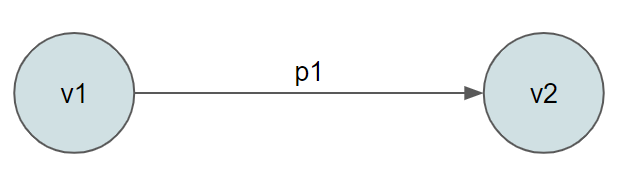
\includegraphics[width=0.5\linewidth]{imagenes/graph1.png}
        \caption{Local index access for a simple graph.}
        \label{fig:example_graph1}
\end{figure}

The graph on \Cref{fig:example_graph1} can be described by the following triple pattern: \texttt{v1 p1 v2}. We consider that each term may be constant or variable. If all the elements are variables, we would let the remote endpoint handle this case (as was described in \Cref{chap:graph_exploration}). For this reason, we will assume that something in this graph is a constant: \texttt{v1}, \texttt{p1} or \texttt{v2}.

Let us consider that \texttt{p1} and \texttt{v2} are variable, but \texttt{v1} is constant. Moreover, let us consider that \texttt{v1} is known to be an instance of type \texttt{Human}.

Let us also consider that we have the following data in our index:
\begin{minted}{csharp}
human1.Properties = [favoriteFood, gender, ...]
human1.Type = [Human]
[...]
human2.Properties = [studiedAt, bornIn, ...]
human2.Type = [Human]
\end{minted}

From the information above, we also know the following for our type \texttt{Human}:
\begin{minted}{csharp}
Human.OutgoingProperties = [favoriteFood, gender, studiedAt, bornIn, ...]
Human.IncomingProperties = [namedAfter, president, author, ...]
[...]
\end{minted}

Given this information, we could provide our users suggestions for \texttt{p1}. This includes properties such as \texttt{favoriteFood}, \texttt{gender}, \texttt{bornIn}, among others.

\end{example}

The previous case shows how we can provide property suggestions for users with no knowledge about the existing structure of a dataset. We would also like to highlight what we have mentioned before about approximated results: since our index is not storing individual triples, but relationships between types, we could provide suggestions that might not be in the original dataset.

Additional to what we could suggest for \texttt{p1}, and given that we have a collection of possible results for \texttt{p1}, we could also infer certain information about the types for \texttt{v2}: instances of the range types for the previous properties, e.g.: instances \texttt{Food}, \texttt{Gender} or \texttt{City}, sorted by relevance.

While this can be costly, the amount of properties in for a large dataset such as Wikidata is around 1300\footnote{The total number of properties are around 8000, but those going from entity-to-entity are only 1300. Other properties go to strings or other datatypes.}, which limits the possibilities for each domain to a few hundred at most. We have decided to also calculate the possible inferred types for \texttt{v2} in this process, since this allow us to provide users with approximate information while building their queries. 

As a summary, for a \texttt{v1 p1 v2} triple pattern, where \texttt{v1} is constant, the following occurs:
\begin{itemize}
    \item The incoming and outgoing properties of all types are indexed.
    \item \texttt{p1} is an outgoing property of the type of \texttt{v1}.
    \item \texttt{v2} is an instance of the range of one of the possible properties for \texttt{p1}.
\end{itemize}

Readers might notice that the previous reasoning would also apply if only \texttt{v2} is constant: we would be able to get suggestions for both \texttt{p1} and \texttt{v1}.

\begin{example}
In the same graph as before, let us now consider that only \texttt{p1} is constant e.g.: \texttt{bornIn}. From our index, we can retrieve both the domain and range for \texttt{bornIn}. 

Let us consider the following values in our index:
\begin{verbatim}
    bornIn.Domain = [Human, Monster, Star, ...]
    bornIn.Range = [City, Hospital, Dungeon, SolarSystem, ...]
\end{verbatim}

Our system will provide suggestions for \texttt{v1} that are instances of \texttt{Human}, \texttt{Monster} or \texttt{Star}, sorted by relevance. The same will occur for \texttt{v2}: instances of \texttt{City}, \texttt{Hospital} or \texttt{Dungeon} could be proposed.

\end{example}

As a summary, for a \texttt{v1 p1 v2} triple pattern, where \texttt{p1} is constant, the following occurs:
\begin{itemize}
    \item The domain and range of all properties are indexed.
    \item \texttt{v1} is an instance of one of the classes in the domain of \texttt{p1}
    \item \texttt{v2} is an instance of one of the classes in the range of \texttt{p1}
\end{itemize}

In our previous example we covered the simplest of all cases. Now we would like to generalize: any node has multiple incoming and outgoing edges.

\begin{example}

Let us consider the graph of \Cref{fig:example_graph2}. 

\begin{figure}[h]
    \centering
        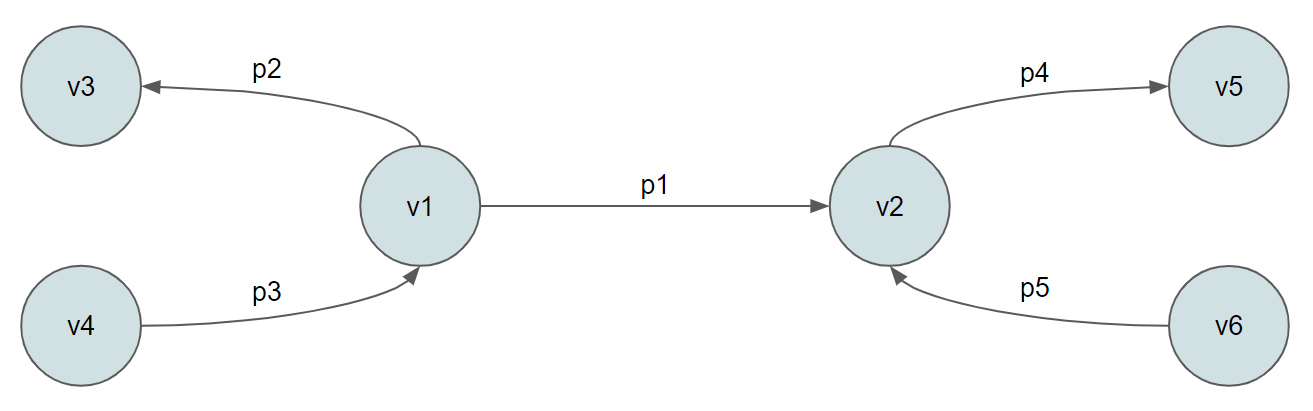
\includegraphics[width=\linewidth]{imagenes/graph2.png}
        \caption{Example graph for expanding domain- and range-types.}
        \label{fig:example_graph2}
\end{figure}

We will consider that any number of elements (nodes or properties) are constant. For each of these constants, we will propagate their types: nodes will contribute with their types to adjacent variable properties; properties will contribute with their domain- and range-types to subject and object variable nodes.

Our first step will be to expand known types among neighbours. The pseudo-code in \Cref{fig:codeExpandNodes} and \Cref{fig:codeExpandEdges} depicts how this task is done for both nodes and properties (i.e., edge labels).

\begin{figure}[h]
\begin{minted}[]{csharp}
// Input:  A query graph with triples as edges;
// Output: The query graph with annotated types for nodes;
//         We will use them to populate our domain and range types (Figure 4.14) 
//         and our edge suggestions (Figure 4.16).
// We refer by DB to our Index database;
ExpandNodes(graph) {
  //We first expand node types:
  foreach(node in graph.Nodes){
    if(node.IsConstant)
      // The DB.GetTypes() method, will query our DB
      // for types (eg.: given Felix, will return Cat)
      node.Types = DB.GetTypes(node);

    //Get types from instanceOf-edges:
    else if(node.IsTyped) 
      // This GetTargetNodeTypes() method will get all types
      // for the instanceOf edges of a node.
      // eg.: given: node - instanceOf - Cow; will return Cow.
      // This applies for multiple instanceOf edges of the node.
      node.Types = graph.GetTargetNodeTypes(node);
  }
}
\end{minted}
\caption{Pseudo-code for expanding node types.}
\label{fig:codeExpandNodes}
\end{figure}

For properties, more logic is required. Checking if the property is constant is not enough, since for example \texttt{bornIn} can have domain \texttt{Human}, \texttt{Cat}, \texttt{Dog}, etc. and range \texttt{City}, \texttt{Hospital}, \texttt{Country}, etc. If in the graph, a specific source type is given, then that type is used instead of the domain, thus further narrowing the available types.

\begin{figure}[h]
\begin{minted}[]{csharp}
// Input:  A query graph with triples as edges;
// Output: The query graph with annotated domain and range types on edges;
//         We will use them to populate our node types (Figure 4.15)
// We refer by DB to our Index database;
ExpandEdges(graph) {
  foreach (edge in graph.Edges) {
    property = edge.Property;
    source = edge.Source;
    target = edge.Target;

    //Source domain types first:
    if(source.IsConstant || source.IsTyped)
      // if the source is given, then the domain are 
      // the types of the source node.
      edge.DomainTypes = source.Types;
    else if(property.IsConstant)
      // Otherwise, get the domains from the DB.
      edge.DomainTypes = DB.GetPropertyDomains(property);

    //Then target range types.
    if(target.IsConstant || target.IsTyped)
      // if the target is given, then the range are 
      // the types of the target node.
      edge.RangeTypes = target.Types;
    else if(property.IsConstant)
      // Otherwise, get the types from the DB.
      edge.RangeTypes = DB.GetPropertyRanges(property);
  }
}
\end{minted}
\caption{Pseudo-code for expanding edge domain- and range-types.}
\label{fig:codeExpandEdges}
\end{figure}

Once we have all known types in place, we can now get values for both nodes and edges. For nodes, we will focus on the outgoing and incoming edges. From these edges, we collect: for the outgoing edges, the domain types (our node must be inside this domain); and for the incoming edges, we collect the range types (our node must also be in this range). In other words, we are going to intersect the outgoing-edges-domain-types and the incoming-edges-range-types. A high-level detail of this process can be appreciated in \Cref{fig:codeResultsNodes}.

\begin{figure}[h]
\begin{minted}[]{csharp}
// Input:  A query graph with triples as edges;
// Output: The query graph with annotated results for suggestions of instances on nodes;
// We refer by DB to our Index database;
GetNodesResults(graph){
  foreach (node in graph.Nodes){
    // We already know what it is, we do not propose suggestions
    if(node.IsConstant) continue;
        
    if(!node.IsTyped) {
      // In practice we initialise types with the types from one of the edges.
      // We present it this way for simplicity.
      node.Types = DB.GetAllTypes();
      
      foreach (outEdge in node.outEdges) {
        if(outEdge.DomainTypes.IsNotEmpty())
            node.Types = Intersect(node.Types, outEdge.DomainTypes);
      }
      foreach (inEdge in node.inEdges) {
        if(inEdge.RangeTypes.IsNotEmpty())
            node.Types = Intersect(node.Types, inEdge.RangeTypes);
      }
    }
    // Finally we get instances for our types.
    // If our node is of a given type, we get instance values:
    // node.IsType = Cat --> node.Results = Simon, Felix, Grumpy, etc.
    // Results will be sorted by relevance and importance.
    node.Results = DB.GetInstancesOf(node.Types);
  }
}
\end{minted}
\caption{Pseudo-code for returning node results.}
\label{fig:codeResultsNodes}
\end{figure}

For edges (\Cref{fig:codeResultsEdges}), we will focus on both the source- and target-node of our edges. We first do some checks on if these nodes are constants or instances of another type. If either our source or target nodes are constant, then we have certainty of the possible values that our edge can have (we recall that we have added these values directly into our DB).

If the source or target node is an instance of another type (thus a variable), then we query the outgoing or incoming properties for that type: while indexing, we have collected these properties for all instances of that type. But in this case, we also explore other possible relations existing in our graph.

Focusing on each node, we will check all outgoing edges with constant properties. Being constant, the properties on these edges can provide information about the values for their domains, and with these, the type of our node. We intersect the domains for all such properties. We will do the same for the incoming edges with constant properties of our source node. If there are such incoming edges, then our node type must be in the range of each of those properties, and thus we again intersect the ranges. Finally, after getting approximate results for both our nodes and edges, a list of entities and properties are now available. 

\begin{figure}[h]
\begin{minted}[]{csharp}
// Input:  A query graph with triples as edges;
// Output: The query graph with annotated results for suggestions of properties on edges;
// We refer by DB to our Index database;
GetEdgesResults(graph){
  foreach(edge in graph.Edges){
    property = edge.Property;
    // We already know what it is, we do not propose suggestions.
    if(property.IsConstant) continue;
    
    source = edge.SourceNode;
    target = edge.TargetNode;

    suggestions = new Set();
    // Properties of the instance (Like outgoing properties for Barack Obama);
    sourceProps = DB.GetOutgoingProperties(source);
    targetProps = DB.GetIncomingProperties(target);
    // Properties of the Type (like outgoing properties of Type Human);
    domainProps = DB.GetPropertiesWithDomainIn(source.Types);
    rangeProps = DB.GetPropertiesWithRangeIn(target.Types);
    if (source.IsConstant && target.IsConstant) {
      suggestions = Intersect(sourceProps, targetProps);
    } else if (source.IsConstant) {
      suggestions = sourceProps;
    } else if (target.IsConstant) {
      suggestions = targetProps;
    } else {
      // In Figure 4.15 we added all types for nodes that had no constants or types.
      suggestions = Intersect(domainProps, rangeProps);
    }
    edge.Results = suggestions;
  }
}
\end{minted}
\caption{Pseudo-code for returning edge results.}
\label{fig:codeResultsEdges}
\end{figure}

\end{example}

Something else that must be mentioned is that for remote queries: both the label and the description are retrieved from the local index and the results are returned to the user. 

% ##############################################################################################
% ##############################################################################################
% ##############################################################################################

\subsection{Approximations}

We have discussed how our system provides suggestions to our users, but we would like to cover the scenario where our system will provide over-approximated results.

\begin{example}
Let us consider the following data:

\begin{minted}[frame=none,linenos=false]{SPARQL}
<uri:/SeattleSlew> <uri:/instanceOf> <uri:/Horse> .
<uri:/SeattleSlew> <uri:/winner> <uri:/KentuckyDerby> .
# [...]
<uri:/Seabiscuit> <uri:/instanceOf> <uri:/Horse> .
<uri:/Seabiscuit> <uri:/sibling> <uri:/Lottery> .
# [...]
\end{minted}

And given the following triple pattern:
\begin{minted}[frame=none,linenos=false]{SPARQL}
?horse <uri:/instanceOf> <uri:/Horse> .
?horse <uri:/winner> ?race .
?horse ?prop ?object .
\end{minted}


In our sample data, only \texttt{Seattle Slew} has the \texttt{winner} property (and no \texttt{sibling} property), but since our data is indexed based on our domain- and range-types, for \texttt{?prop}, we will also get \texttt{sibling} as a suggestion property, although our data has no triples with both properties there.

\end{example}

% ##############################################################################################
% ##############################################################################################
% ##############################################################################################

\section{Application Interface}
\label{chap:api}

The last module of our system is the application interface. It will allow our system to take requests from front-end clients and use our backend.

As was mentioned before, our system supports several types of requests:
\begin{itemize}
    \item Keyword search for entities.
    \item Keyword search for properties.
    \item Keyword search for types.
    \item Get information about a Q-code entity: label, description, etc.
    \item Get information about a P-code property: label, description, etc.
    \item Query term with a SPARQL query text.
    \item Query term with a graphical representation of a SPARQL query.
\end{itemize}

The keyword search directly reverts to the specialized index. The query term works as was previously described in this chapter.

With all of these components in place, our backend can accept and respond to requests from a frontend client. In the following chapter we will describe how to integrate our system with RDFExplorer as the client in order to apply our approach for a concrete use-case.


